\section{Analysis}
\label{sec:analysis}

\subsection{Representation structure}

The decisive observation is the split between exact-token and downstream metrics. v4 loses 0.32 points of free-running acoustic top-1 against v2 and gains 0.105 of replay cosine; its 5th-percentile track beats the best v2 or v3 track. This suggests substantial functional redundancy in the code space: many code tuples appear to map to similar condition embeddings, and an encoder can be functionally close while disagreeing with the one tuple the generator happened to sample. Exact agreement is bounded by that sampling, not by the encoder, which is consistent with the semantic head saturating near 43\% top-1 and 80\% top-5 across every model while replay keeps improving. We have not quantified equivalence classes of tuples directly; the claim rests on the divergence of the two metrics.

Table~\ref{tab:forcing} makes the same point from inside the v4 model by scoring it under the two conditions it can be run in. Free-running, the first numeric column, is the inference condition: each acoustic head sees the greedy predictions of the heads below it. Teacher-forced, the second column, is the training condition: each head sees the sampled codes below it. The two semantic rows are identical, because the semantic readout does not depend on the acoustic codes. The two acoustic rows differ by a factor of 2.5 at top-1 (7.3\% against 18.4\%) and 2.2 at top-5 (19.9\% against 44.6\%): the decoder has learned the conditional structure of the codebooks, and feeding back its own earlier choices is what costs exact agreement. Since the replay cosine of Tab.~\ref{tab:replay} is measured on the free-running codes, the 0.8748 is achieved with the 7.3\% column, not the 18.4\% one.

\begin{table}[tb]
\centering
\small
\caption{v4 at the final checkpoint, free-running against teacher-forced (percent).}
\label{tab:forcing}
\adjustbox{max width=\columnwidth}{
\begin{tabular}{lrr}
\toprule
Metric & Free-running & Teacher-forced \\
\midrule
semantic top-1 & 43.17 & 43.17 \\
semantic top-5 & 80.51 & 80.51 \\
acoustic top-1 & 7.29 & 18.42 \\
acoustic top-5 & 19.88 & 44.55 \\
\bottomrule
\end{tabular}
}
\end{table}


\subsection{RVQ codebook behaviour}

Because the codebook entries are never observed, the codebooks can only be characterised by how predictable each one is from audio. Table~\ref{tab:depth} gives top-1 agreement for every codebook separately at the matched step 17,500. The first column is the codebook index, with 0 the semantic stream and 1 to 7 the acoustic residuals in order of depth; the next three columns are the independent-head models v1, v2 and v3; the last two are v4 free-running and v4 teacher-forced. Reading down any of the first three model columns shows the depth gradient: from 11 to 12\% at codebook 1 to under 3\% at codebook 7, and the three columns differ by at most 0.7 points at any depth. Reading down the teacher-forced column shows what the decoder learned, 27.0\% at codebook 1 and still 11.9\% at codebook 7, more than four times the independent heads at depth. The free-running column sits above v3 at codebooks 1 and 2 and falls below it from codebook 4 on, where an early disagreement has propagated through the conditioning.

\begin{table}[tb]
\centering
\small
\caption{Top-1 agreement by codebook at step 17,500 (percent).}
\label{tab:depth}
\adjustbox{max width=\columnwidth}{
\begin{tabular}{lrrrrr}
\toprule
Codebook & v1 & v2 & v3 & v4 free-running & v4 teacher-forced \\
\midrule
0 & 41.03 & 42.86 & 43.03 & 43.16 & 43.16 \\
1 & 11.27 & 11.96 & 12.04 & 14.72 & 27.04 \\
2 & 11.92 & 12.56 & 12.62 & 13.02 & 24.49 \\
3 & 9.34 & 10.00 & 9.98 & 9.46 & 19.32 \\
4 & 7.54 & 8.07 & 8.17 & 6.56 & 16.66 \\
5 & 4.45 & 4.71 & 4.74 & 3.41 & 15.46 \\
6 & 3.08 & 3.29 & 3.26 & 2.16 & 14.10 \\
7 & 2.58 & 2.77 & 2.77 & 1.76 & 11.88 \\
\bottomrule
\end{tabular}
}
\end{table}


The monotone decline of the independent heads is consistent with the conditional dependence induced by residual quantisation, where deeper codebooks refine a representation determined by the codes below and an independent head cannot see which were chosen. Under greedy feedback most of the teacher-forced gain is lost in exact agreement, the exposure bias of sequence models~\cite{bengio2015scheduled,ranzato2016sequence} across depth rather than time. The replay metric suggests that many of the alternative tuples remain functionally compatible with the generator: although they differ from the sampled tuple, they induce substantially more similar conditioning than exact-token agreement implies.

\subsection{Musical information across levels}

Figure~\ref{fig:depth} plots the seven acoustic columns of Tab.~\ref{tab:depth} against codebook index. The three solid curves of the independent-head models lie on top of one another, which is the visual form of the width and MERT ablations having no effect on the depth gradient. The dashed curve is the teacher-forced v4 decoder, the conditional structure it learned; the solid v4 curve is what survives greedy decoding, and the vertical distance between the two at each codebook is the exposure gap, widening from 12 points at codebook 1 to 10 points at codebook 7 while both curves fall. The figure also shows where the free-running v4 curve crosses below the independent heads, between codebooks 3 and 4.

\begin{figure}[tb]
  \centering
  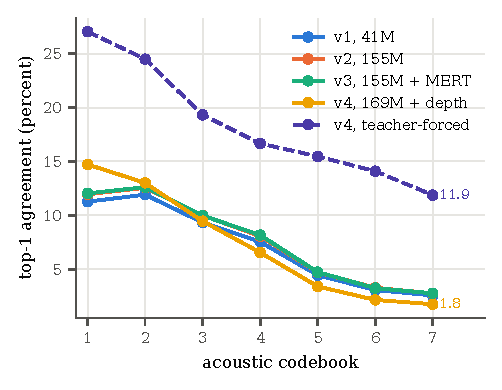
\includegraphics[width=\columnwidth]{figures/depth_gradient.pdf}
  \caption{Top-1 agreement by acoustic codebook at step 17,500. Independent heads (v1 to v3) collapse with depth; the depth-causal decoder (v4) does not when teacher-forced and partly does under greedy feedback.}
  \label{fig:depth}
\end{figure}

The semantic codebook is the most predictable stream from audio (43\% top-1, 80\% top-5 over 16,384 entries) and the one the language model plans directly; it carries the content that a text prompt determines. The acoustic codebooks refine timbre and detail and are progressively less determined by the audio alone: given the codes below, codebook 1 is predicted at 27\% and codebook 7 at 12\%, and without them the later books approach chance. Width and MERT alignment, both of which enrich the frame representation, barely move any level; conditioning across levels moves all of them. The information that matters appears to lie in the joint structure of the tuple rather than in any level in isolation.

\subsection{Implications for generative modelling}

For reference-conditioned generation the practical recipe follows from the analysis: constrain the semantic stream, which the encoder predicts well and which the language model consumes directly, and let the generator draw the acoustic codes itself. The released integration restricts every fifth generated semantic code to the encoder's top-5 candidates and generates all seven acoustic codebooks with the official depth decoder. More generally, an encoder for a hierarchical code space should be scored by what the downstream model does with its codes, and should decode across depth rather than read levels independently.
